\chapter{Controlling program flow}
\label{chap:flow}
Non-recursive functions encapsulates code and allows for some control of flow, that is, if there is a piece of code, which we need to to have executed many times, then we can encapsulate it in the body of a function, and then call the function several times. In this chapter, we will look at more general control of flow via loops, conditional execution, and recursion, and therefore we look at further extension of the \lstinline[language=ebnf]!expr! rule,
\begin{verbatimwrite}{tmp.ebnf}
expr = ... 
  | "if" expr "then" expr {"elif" expr "then" expr} ["else" expr] (*conditional*)
  | "while" expr "do" expr ["done"] (*while loop*)
  | "for" ident "=" expr "to" expr "do" expr ["done"] (*simple for loop*)
  | "let" functionDefn "in" expr (*binding a function or operator*)
  | "let" "rec" functionDefn {"and" functionDefn} "in" expr (*recursive fcts*)
\end{verbatimwrite}
\ebnf{tmp.ebnf}{Expressions for controlling the flow of execution.}

\section{For and while loops}
Many programming constructs need to be repeated, and F\# contains many structures for repetition such as the \keyword{for} and \keyword{while} loops, which have the syntax,
%
\begin{verbatimwrite}{tmp.ebnf}
expr = ... 
  | "while" expr "do" expr ["done"] (*while loop*)
  | "for" ident "=" expr "to" expr "do" expr ["done"] (*simple for loop*)
\end{verbatimwrite}
\ebnf{tmp.ebnf}{\lstinline{for}- and \lstinline{while}-loops.}
%
As an example, consider counting from 1 to 10 with a \idx{\keyword{for}}-loop,
%
\fsOutput{count}{Counting from 1 to 10 using a \keyword{for}-loop.}
%
As this interactive script demonstrates, the identifier \lstinline!i! takes all the values between 1 and 10, but in spite of its changing state, it is not mutable. Note also that the return value of the \keyword{for} expression is \lexeme{()} like the \lstinline!printf! functions. 
Using lightweight syntax the block following the \idx{\keyword{do}} keyword up to and including the \idx{\keyword{done}} keyword may be replaced by a newline and indentation, e.g.,
%
\fs{countLightweight}{Counting from 1 to 10 using a \keyword{for}-loop, see Listing~\ref{count}.}
%
A more complicated example is,
\begin{problem}
  Write a program that calculates the $n$'th Fibonacci number.
\end{problem}
The Fibonacci numbers is the series of numbers $1,1,2,3,5,8,13\dots$, where the $\text{fib}(n) = \text{fib}(n-1)+\text{fib}(n-2)$, and they are related to Golden spirals shown in Figure~\ref{fig:goldenSpiral}.
\begin{figure}
  \centering
  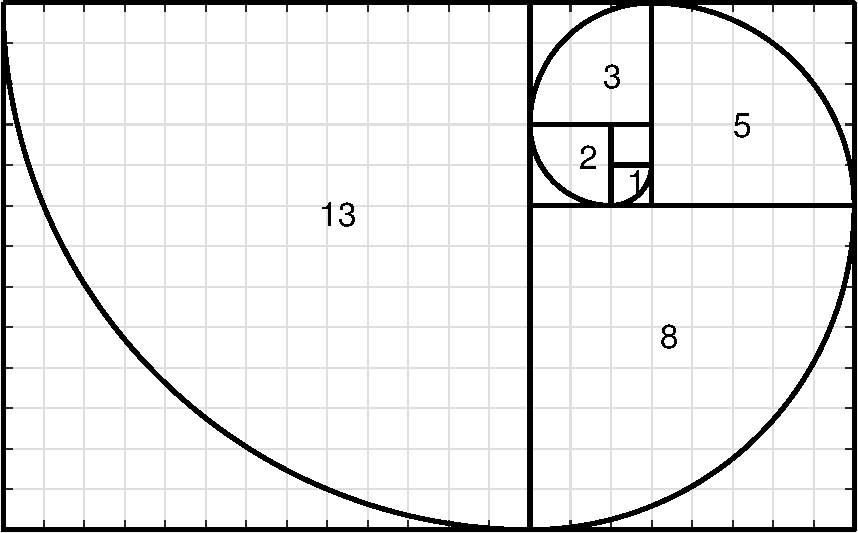
\includegraphics[width=0.45\linewidth]{Fibonacci_spiral}
  \caption{The Fibonacci spiral is an approximation of the golden spiral. Each square has side lengths of successive Fibonacci numbers, and the curve in each square is the circular arc with radius of the square it is drawn in}
  \label{fig:goldenSpiral}
\end{figure}
We could solve this problem with a \keyword{for}-loop as follows,
%
\fs{fibFor}{The $n$'th Fibonacci number is the sum of the previous 2.}
%
The basic idea of the solution is that if we are given the $(n-1)$'th and $(n-2)$'th numbers, then the $n$'th number is trivial to compute. And assume that $\text{fib}(1)$ and $\text{fib}(2)$ are given, then it is trivial to calculate the $\text{fib}(3)$. For the $\text{fib}(4)$ we only need $\text{fib}(3)$ and $\text{fib}(2)$, hence we may disregard $\text{fib}(1)$. Thus we realize, that we can cyclicly update the previous, current and next values by shifting values until we have reached the desired $\text{fib}(n)$.

\begin{comment}
  For the alternative \keyword{for}-loop, consider the problem,
  \begin{problem}
    Write a program that identifies prime factors of a given integer $n$.
  \end{problem}
  Prime numbers are integers divisible only be 1 and themselves with zero remainder. Let's assume that we already have identified a list of primes from 2 to $n$, then we could write a program that checks the remainder as follows,
  % 
  \fs{primeCheck}{Checking whether a given number has remainder zero after division by some low prime numbers.}
  % 
  In this example, the variable \lstinline!i! runs through the elements of a list, which will be discussed in further detail in  Chapter~\ref{chap:lists}.
\end{comment}

The \idx{\keyword{while}}-loop is simpler than the \keyword{for}-loop and does not contain a builtin counter structure. Hence, if we are to repeat the count-to-10 program from Listing~\ref{count} example, it would look somewhat like,
%
\fs{countWhile}{Count to 10 with a counter variable.}
%
or equivalently using the lightweight syntax,
%
\fs{countWhileLightweight}{Count to 10 with a counter variable using lightweight syntax, see Listing~\ref{countWhile}.}
%
In this case, the \keyword{for}-loop is to be preferred, since more lines of code typically means more chances of making a mistake. But the \keyword{while}-loop allows for other logical structures. E.g., lets find the biggest Fibonacci number less than 100,
%
\fs{fibWhile}{Search for the largest Fibonacci number less than a specified number.}
%
Thus, \keyword{while}-loops are most often used, when the number of iteration cannot easily be decided, when entering the loop.

Both \keyword{for}- and \keyword{while}-loops are often associated with variables, i.e., values that change while looping. If one mistakenly used values and rebinding, then the result would in most cases be of little use, e.g.,
%
\fs{forScopeError}{Lexical scope error. While rebinding is valid F\# syntax, has little effect due to lexical scope.}
%
I.e., the \keyword{let} expression rebinds \lstinline!a! every iteration of the loop, but the value on the right-hand-side is taken lexically from above, where \lstinline!a! has the value 1, so every time the result is the value 2.

\section{Conditional expressions}
Consider the task,
\begin{problem}
  Write a function that given $n$ writes the sentence, ``I have n apple(s)'', where the plural 's' is added appropriately.
\end{problem}
For this we need to test the value of $n$, and one option is to use conditional expressions. Conditional expression has the syntax,
%
The grammar for conditional expressions is,
\begin{verbatimwrite}{tmp.ebnf}
expr = ... 
  | "if" expr "then" expr {"elif" expr "then" expr} ["else" expr] (*conditional*)
\end{verbatimwrite}
\ebnf{tmp.ebnf}{Conditional expressions.}
%
and an example using conditional expressions to solve the above problem is,
%
\fs{conditionalLightweight}{Using conditional expression to generate different strings.}
%
The \lstinline[language=ebnf]!expr! following \idx{\keyword{if}} and \idx{\keyword{elif}} are \idx{conditions}, i.e., expressions that evaluate to a boolean value. The \lstinline[language=ebnf]!expr! following \idx{\keyword{then}} and \idx{\keyword{else}} are called \idx{branches}, and all branches must have identical type, such that regardless which branch is chosen, then the type of the result of the conditional expression is the same. The result of the conditional expression is the first branch, for which its condition was true. 

The sentence structure and its variants gives rise to a more compact solution, since the language to be returned to the user is a variant of "I have/or no/number apple(s)", i.e., under certain conditions should the sentence use ``have'' and ``owe'' etc.. So we could instead make decisions on each of these sentence parts and then built the final sentence from its parts. This is accomplished in the following example:
%
\fs{conditionalLightweightAlt}{Using sentence parts to construct the final sentence.}
%
While arguably shorter, this solution is also more dense, and for a small problem like this, it is most likely more difficult to debug and maintain.

Note that both \keyword{elif} and \keyword{else} branches are optional, which may cause problems. For example, both \mbox{\lstinline!let a = if true then 3!} and \mbox{\lstinline!let a = if true then 3 elif false then 4!}  will be invalid, since F\# is not smart enough to realize that the type of the expression is uniquely determined. Instead F\# looks for the \keyword{else} to ensure all cases have been covered, and that \lstinline!a! always will be given a unique value of the same type regardless of the branches taken in the conditional statement, hence, \mbox{\lstinline!let a = if true then 3 else 4!}  is the only valid expression of the 3. In practice, F\# assumes that the omitted branches returns \lexeme{()}, and thus it is fine to say \mbox{\lstinline!let a = if true then ()!} and \mbox{\lstinline!if true then printfn "hej"!}. Nevertheless, it is good practice in F\# always to include and \keyword{else} branch.


% since in, e.g., \keyword{let} expressions, F\# requires all cases to be covered, 

% A basic flow control mechanism used both for functional and imperative programming is the \lstinline{if-then-else} construction, e.g.,
% \fs{flowIfThen}{}
% I.e., if and only if the value of the argument is postive, then it will be printed on screen. More common is to include the \lstinline{else} 
% \fs{flowIfThenElse}{}
% A common construction is a nested list of \lstinline{if-then-else},
% \fs{flowIfThenElseNested}{}
% where the integers 0--2 are converted to characters, and integers outside this domain is converted to the nearest equivalent number. This construction is so common that a short-hand notation exists, and we may equivalently have written,
% \fs{flowIfThenElseNestedShort}{}

\section{Recursive functions}
Recursion is a central concept in F\#. A \idx{recursive function} is a function, which calls itself. From a compiler point of view, this is challenging, since the function is used before the compiler has completed its analysis. However, for this there is a technical solution, and we will just concern ourselves with the logics of using recursion for programming. The syntax for defining recursive functions in F\# is,
%
\begin{verbatimwrite}{tmp.ebnf}
expr = ... 
  | "let" "rec" functionDefn {"and" functionDefn} "in" expr
\end{verbatimwrite}
\ebnf{tmp.ebnf}{Recursive functions.}
%
An example of a recursive function that counts from 1 to 10 similarly to Listing~\ref{count} is,\jon{A drawing showing the stack for the example would be good.}
%
\fs{countRecursive}{Counting to 10 using recursion.}
%
Here the \lstinline!prt! calls itself repeatedly, such that the first call is \lstinline!prt 1 10!, which calls \lstinline!prt 2 10!, and so on until the last call \lstinline!prt 10 10!. Calling \lstinline!prt 11 10! would not result in recursive calls, since when \lstinline!a! is higher than \lstinline!10! then the \idx{stopping criterium} is met and a newline is printed. For values of \lstinline!a! smaller than or equal \lstinline!b! then the recursive branch is executed. Since \lstinline!prt! calls itself at the end of the recursion branch, then this is a \idx{tail-recursive} function. Most compilers achieve high efficiency in terms of speed and memory, so \advice{prefer tail-recursion whenever possible.}
Using recursion to calculate the Fibonacci number as Listing~\ref{fibFor}.
%
\fs{fibRecursive}{The $n$'th Fibonacci number using recursive.}
%
Here we used the fact that including $\text{fib}(0)=0$ in the Fibonacci series also produces it using the rule $\text{fib}(n)=\text{fib}(n-2)+\text{fib}(n-1),\; n\geq 0$, which allowed us to define a function that is well defined for the complete set of integers. I.e., a negative argument returns 0. This is a general advice: \advice{make functions that fails gracefully.} 
%The recursive definition allows for recursive value definitions and defining several values and functions in one expression. Recursive values is particularly useful for defining infinite sequences, see Section~\ref{sec:sequences}.

Functions that recursively call each other are called \idx{mutually recursive} functions. F\# offers the \mbox{\keyword{let}-\keyword{rec}-\keyword{and}} notation for co-defining mutually recursive functions. As an example, consider the function \mbox{\lstinline!even : int -> bool!}, which returns true if its argument is even and false otherwise, and the opposite function \mbox{\lstinline!odd : int -> bool!}. A mutually recursive implementation of these functions can be developed from the following statements: \mbox{\lstinline!even 0 = true!}, \mbox{\lstinline!odd 0 = false!}, and \mbox{\lstinline!even n = odd (n-1)!}: 
%
\fs{mutuallyRecursive}{Using mutual recursion to implement even and odd functions.}
%
Notice that in the lightweight notation used here, that the \keyword{and} must be on the same indentation level as the original \keyword{let}.

Without the \keyword{and} keyword, F\# will return an error at the definition of \lstinline!even!. However, it is possible to implement mutual recursion by using functions as an argument, e.g.,
%
\fs{mutuallyRecursiveAlt}{Mutual recursion without the \keyword{and} keyword needs a helper function.}
%
But, Listing~\ref{mutuallyRecursive} is clearly to be preferred over Listing~\ref{mutuallyRecursiveAlt}. 

In the above we used the \lstinline!even! and \lstinline!odd! function problems to demonstrate mutual recursion. There is, of course, a much simpler solution, which does not use recursion at all:
%
\fsCode{parity}{parity}{A better way to test for parity without recursion.}{}
%
which is to be preferred anytime as the solution to the problem.

\section{Programming intermezzo}
Using loops and conditional expressions we are now able to solve the following problem
\begin{problem}
  Given an integer on decimal form, write its equivalent value on binary form
\end{problem}
To solve this problem, consider odd numbers: They all have the property, that the least significant bit is 1, e.g., $1_2 = 1, 101_2 = 5$ in contrast to even numbers such as $110_2 = 6$. Division by 2 is equal to right-shifting by 1, e.g., $1_2/2 = 0.1_2 = 0.5, 101_2/2 = 10.1_2 = 2.5, 110_2/2 = 11_2 = 3$. Thus by integer division by 2 and checking the remainder, we may sequentially read off the least significant bit. This leads to the following algorithm,
%
\fs{dec2bin}{Using integer division and remainder to write any positive integer on binary form.}
%
Another solution is to use recursion instead of the \keyword{while} loop:
%
\fs{dec2binRec}{Using recursion to write any positive integer on binary form, see also Listing~\ref{dec2bin}.}
%
Listing~\ref{dec2bin} is a typical imperative solution, where the states \lstinline!v! and \lstinline!str! are iteratively updated until \lstinline!str! finally contains the desired solution. Listing~\ref{dec2binRec} is a typical functional programming solution, to be discussed in Part~\ref{part:declarative}, where the states are handled implicitly as new scopes created by recursively calling the helper function. Both solutions have been created using a local helper function, since both solutions require special treatment of the cases $n<0$ and $n=0$. 

Let us compare the two solutions more closely: The computation performed is the same in both solutions, i.e., integer division and remainder is used repeatedly, but since the recursive solution is slightly shorter, then one could argue that it is better, since shorter programs typically have fewer errors. However, shorter program also typically means that understanding them is more complicated, since shorter programs often rely on realisations that the author had while programming, which may not be properly communicated by the code nor comments. Speedwise, there is little difference between the two methods: 10,000 conversions of \lstinline!System.Int32.MaxValue!, i.e., the number 2,147,483,647, takes about 1.1 sec for both methods on an 2,9 GHz Intel Core i5 machine.

Notice also, that in Listing~\ref{dec2binRec}, the prefix \lstinline!"0b"! is only written once. This is advantageous for later debugging and updating, e.g., if we later decide to alter the program to return a string without the prefix or with a different prefix, then we would only need to change one line instead of two. However, the program has gotten slightly more difficult to read, since the string concatenation operator and the \lstinline!if! statement are now intertwined. There is thus no clear argument for preferring one over the other by this argument.

Proving that Listing~\ref{dec2binRec} computes the correct sequence is easily done using the induction proof technique: The result of \lstinline!dec2binHelper 0! is clearly an empty string. For calls to \lstinline!dec2binHelper n! with $n>0$, we check that the right-most bit is correctly converted by the remainder function, and that this string is correctly concatenated with \lstinline!dec2binHelper! applied to the remaining bits. A simpler way to state this is to assume that \lstinline!dec2binHelper! has correctly programed, so that in the body of \lstinline!dec2binHelper!, then recursive calls to \lstinline!dec2binHelper! returns the correct value. Then we only need to check that the remaining computations are correct. Proving that Listing~\ref{dec2bin} calculates the correct sequence essentially involves the same steps: If $v = 0$ then the \keyword{while} loop is skipped, and the result is the initial value of \lstinline!str!. For each iteration of the \keyword{while} loop, assuming that \lstinline!str! contains the correct conversions of the bits up till now, we check that the remainder operator correctly concatenates the next bit, and that \lstinline!v! is correctly updated with the remaining bits. We finally check that the loop terminates, when no more 1-bits are left in \lstinline!v!. Comparing the two proofs, the technique of assuming that the problem has been solved, i.e., that recursive calls will work, helps us focus on the key issues for the proof. Hence, we conclude that the recursive solution is most elegantly proved, and thus preferred.

% Functions may be declared using pattern matching, which is a flexible method for declaring output depending on conditions on the input value. The most common pattern matching method is by use of the \lstinline{match with} syntax,
% \fs{functionDeclarationMatchWith}{}

% A short-hand only for functions of 1 parameter is the \lstinline{function} syntax,
% \fs{functionDeclarationFunction}{}
% Note that the name given in the match, here \lstinline{n}, is not used in the first line, and is arbitrary at the line of pattern matchin, and may even be different on each line. For these reasons is this syntax discouraged.

%%% Local Variables:
%%% TeX-master: "fsharpNotes"
%%% End:
